\subsection{Simulated TCEs}
\label{s:simulated}
In order to measure the performance of the Robovetter and the \Kepler\ Pipeline, we created simulated transits and simulated false alarms. The simulated transits are created by injecting transit signals onto the pixels of our original data. The simulated false alarms were created in two separate ways: by inverting the light curves, and by scrambling the sequence of cadences in the time series. 

%For both the \invtce{s} and the \scrtce{s} we needed to remove true astrophysical events, as explained in \S\ref{s:clean} below, in order to match the false alarms found in the \opstce data set.
%JLC1: I think the final sentence is confusing extra detail in the intro paragraph to this section. % SEM Agreed.

\subsubsection{True Transits -- Injection}
\label{injectsec}

We empirically measure the completeness of the \Kepler\ pipeline by injecting a suite of simulated transiting planet signals into the calibrated pixel data and observing their recovery, as was done for previous versions of the pipeline by \citep{Christiansen2013a,Christiansen2015,Christiansen2016}. The full DR25 analysis is described in detail in \citep{Christiansen2017}; the analysis in this paper relied on the on-target injections (Group 1) in that document. We briefly describe their properties here for completeness. For each of 146,294 targets, we generate a model transit signal using the \citet{Mandel2002} formulation, with parameters drawn from the following uniform distributions: orbital periods from 0.5--500 days (0.5--100 days for M dwarf targets), planet radii from 0.25-7 R$_{\odot}$ (0.25-4 R$_{\odot}$ for M dwarf targets), and impact parameters from 0--1. After some re-distribution in planet radius to ensure sufficient coverage from the pipeline being fully incomplete (0~per cent recovery) to fully complete (100~per cent recovery), we find that 50~per cent of the injections have planet radii below 2 R$_{\odot}$ and 90~percent below 40 R$_{\odot}$. The signals are injected into the calibrated pixels, and then processed through the remaining components of the \Kepler\ pipeline in an identical fashion to the original data. Any detected signals are subjected to the same scrutiny by the pipeline and the Robovetter as the original data. By measuring the rate of successful Pipeline recovery and robovetter disposition of signals at a given orbital period and planet radius, we can then correct the number of candidates found at that period and radius to the number that are truly in the data. %SEM: True planets could imply other completeness factors like the inclination.  I think this clarifies.


\subsubsection{False Alarms -- Inverted and Scrambled} 

To create realistic false alarms which have noise properties similar to our \opstce{s}, we inverted the light curves (i.e. multiplied the normalized flux values by negative one) before searching for transit signals. Because the pipeline is only looking for transit-like (negative) dips in the light curve, the true exoplanet transits should no longer be found. However, periodic instrumental and stellar noise will be found. This approach assumes that the sources of false alarms are symmetric in relative flux. The period distribution of these \invtce{s} is shown in Figure~\ref{f:simtces}. The distribution with period of these events qualitatively emulates those seen in the \opstce s; however there are only $\sim$60\% as many. The one-year spike is clearly seen, but is not as tall as we might expect given the size of the one-year spike in the \opstce\ period distribution. 

Another method to create false alarms is to scramble the order of the data. The requirement is to scramble the data enough to lose the coherency of the binary stars and exoplanet transits, but to keep the coherency of the instrumental and stellar red noise that plagues the \Kepler\ data set. Our final solution was to scramble the data in coherent chunks of one year. The fourth year of data (Q13--Q16) was moved to the start of the light curve, followed by the third year (Q9--Q12), the second (Q5--Q8), and the first (Q1--Q4). Q17 remained at the end of the light curve. Within each year, the order of the data did not change. Notice that in this configuration each quarter remains in the correct \Kepler\ season.
%SEM it doesn't actually recreate the rolling band, one year spike, so I don't like this clause  ; this leads to the desired preservation of the false alarms caused by the yearly, rolling-band artifacts \citep{KIH}.

\begin{figure}[h!]
 \begin{center}
  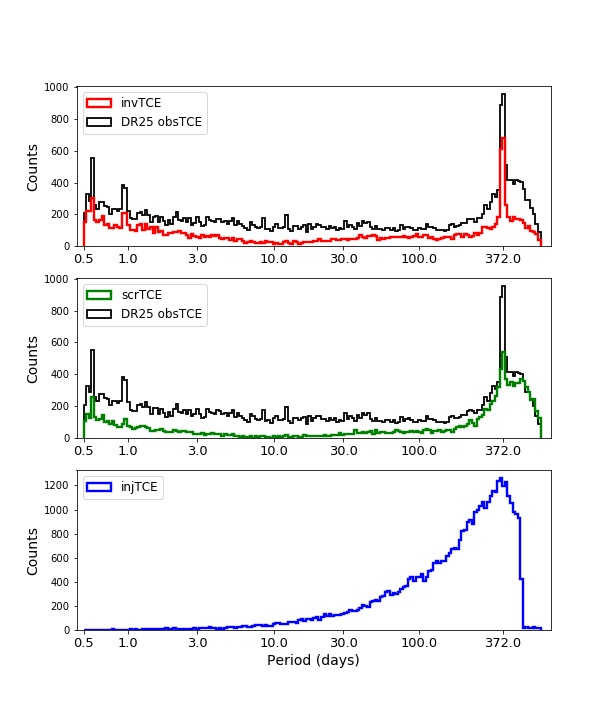
\includegraphics[width=1.0\linewidth]{fig-simulTcePeriods.png}
  \caption{Histogram of the log$_{10}$(period) in days of the \invtce{s} (top, red), the \scrtce{s} (middle, green) and \injtce{s} (bottom, black). The DR25 \opstce{s} are shown for comparison on the top two figures in black.  At shorter periods ($< 30$\,days), the difference between the simulated false alarm sets and the observed data represents the number of transit-like KOIs, at longer periods we primarily expect false alarms.  Notice that the \invtce{s} do a better job of reproducing the one-year spike, but the \scrtce{s} reproduce the long period hump better. Also, notice that the recovered \injtce{s} are dominated by long period events. }
  \label{f:simtces} 
 \end{center}
 \end{figure}

%In Figure~\ref{f:false} we show an example of the folded light curves of an \opstce, \invtce, and \scrtce\ where the number of identified transit events is three.  Notice that for low signal-to-noise \Kepler\ data is capable of having three events due to noise line-up and produce something that looks very similar to an exoplanet transit.  

\subsubsection{Cleaning Inversion and Scrambling}
\label{s:clean}
As described in \S\ref{s:relcalc}, we want to use the \invtce\ and \scrtce\ sets to measure the reliability of the DR25 catalog against instrumental and stellar noise. In order to do that well, we need to remove signals found in these sets that are not typical of those in our \opstce\ set. For inversion, there are astrophysical events that look similar to an inverted eclipse, for example the self-lensing binary star, K03278.01 \citep{Kruse2014}, and Heartbeat binaries \citep{Thompson2012}. With the assistance of published systems and early runs of the Robovetter, we identified any \invtce\ that could be identified as possibly one of these types of astrophysical events; 54 systems were identified in total. Also, the shoulders of inverted eclipsing binary stars and high signal-to-noise KOIs are found by the pipeline but are not the type of false alarm we were trying to reproduce, since they have no corresponding false alarm in the original, un-inverted light curves. We remove any \invtce{s} that were found on stars that had 1) one of the identified astrophysical events, 2) a detached eclipsing binary listed in \citet{Kirk2016} with morphology values larger than 0.6, or 3) a known KOI.  This results in \ninvtces\ \invtce s; their distribution is plotted in Figure~\ref{f:simtces}.

For season scrambling, we do not have to worry about the astrophysical events that emulate inverted transits, but we do have to worry about triggering on true transits that have been rearranged to line up with noise. For this reason we remove from the \scrtce\ population all that were found on a star with a known eclipsing binary \citep{Kirk2016}, or on a previously identified KOI. The result is \nscrtces\ \scrtce s; their distribution is plotted in Figure~\ref{f:simtces}. 

After cleaning the \invtce s and \scrtce s of the eclipsing binary and KOI systems, the number of \scrtce s at periods longer than 200\,d closely matches the size and shape of the same period range in the \opstce s, except for the one-year spike.  The one-year spike is well represented by the \invtce s.  Combining the two sets appears to give us a good handle on the type and relative frequency of false alarms present in our \opstce\ population. Table\,\ref{tab:invscr} lists those \invtce{s} and \scrtce{s} that we used when calculating the effectiveness and reliability of the catalog.

%\subsection{How good are the simulated data sets}
%We should show some evidence that the fraction of false alarms in the simulated data sets matches those in the actual OBS data.  Can we show that the fraction of fails by LPP, individual transits and sig-pri/Fred are approximately the same between the two sets.  Or how different are they.  Do this for low mes,

[MISSING: Table Listing those KICs we cleaned away]

%\subsubsection{Other Simulated sets}
%We also simulated other types of false positives through transit injection \citep{Christiansen2017}. A portion of the injections were injected off the target by less than a pixel.  This is a way of testing our ability to find background eclipsing binaries by looking for small shifts in the location of the transit compared to the location of the target star.  Also, we injected two transits on some stars to emulate an eclipsing binary and test our tools to identify the presence of a significant secondary eclipse.  However because the majority of our false positives are caused by instrumental noise, and because the size of the astrophysical false positive reliability has been well characterized for \Kepler\ \citep[e.g.][]{Morton2016}, we limit our reliability discussion to those caused by instrumental and stellar noise. 


%All of the data sets described above are available in their entirety at the NASA Exoplanet Archive.  All of the metrics described in \S\ref{s:robovetter} to evaluate the disposition of these TCEs are also available in the same table. 